\chapter{Architecture}
\label{ch:architecture}
Slips is modular software. Each module is designed to perform a specific detection in the network traffic.\cite{slips}
In addition to that, the modules can be also used to directly extend Slips with any additional functionality. 
Fides was designed for seamless interoperability with Slips and in addition to the generic trust model, we developed the Fides module for Slips.
In this chapter, we describe the architecture of Fides, and how it interacts with the network as well as with Slips.

\begin{figure}[ht]
    \centering
    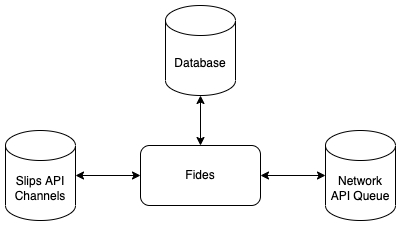
\includegraphics[width=0.7\textwidth]{assets/high_architecture.png}
    \caption{High-Level Architecture}
    \label{fig:high-level-architecture}
\end{figure}

From the high-level perspective (see figure~\ref{fig:high-level-architecture}), the trust model communicates with two different entities - Slips and the network layer.
For both parts, Fides exposes and consumes an API~\cite{api} that is built using the Redis channels.
The messages and API calls are consumed using JSON~\cite{json} data format.

Redis is an in-memory data structure store that supports asynchronous channels and a publish-subscribe model \cite{redis}.
We choose to employ Redis channels, as the medium that allows communication between the network layer and Fides and allows them to use their respective APIs because Slips already uses Redis for its internal communication between modules, it brings no additional overhead to run Fides with its network layer.

\section{Fides \& Network Access}
\label{sec:fides-and-network-access}

\begin{figure}[ht]
    \centering
    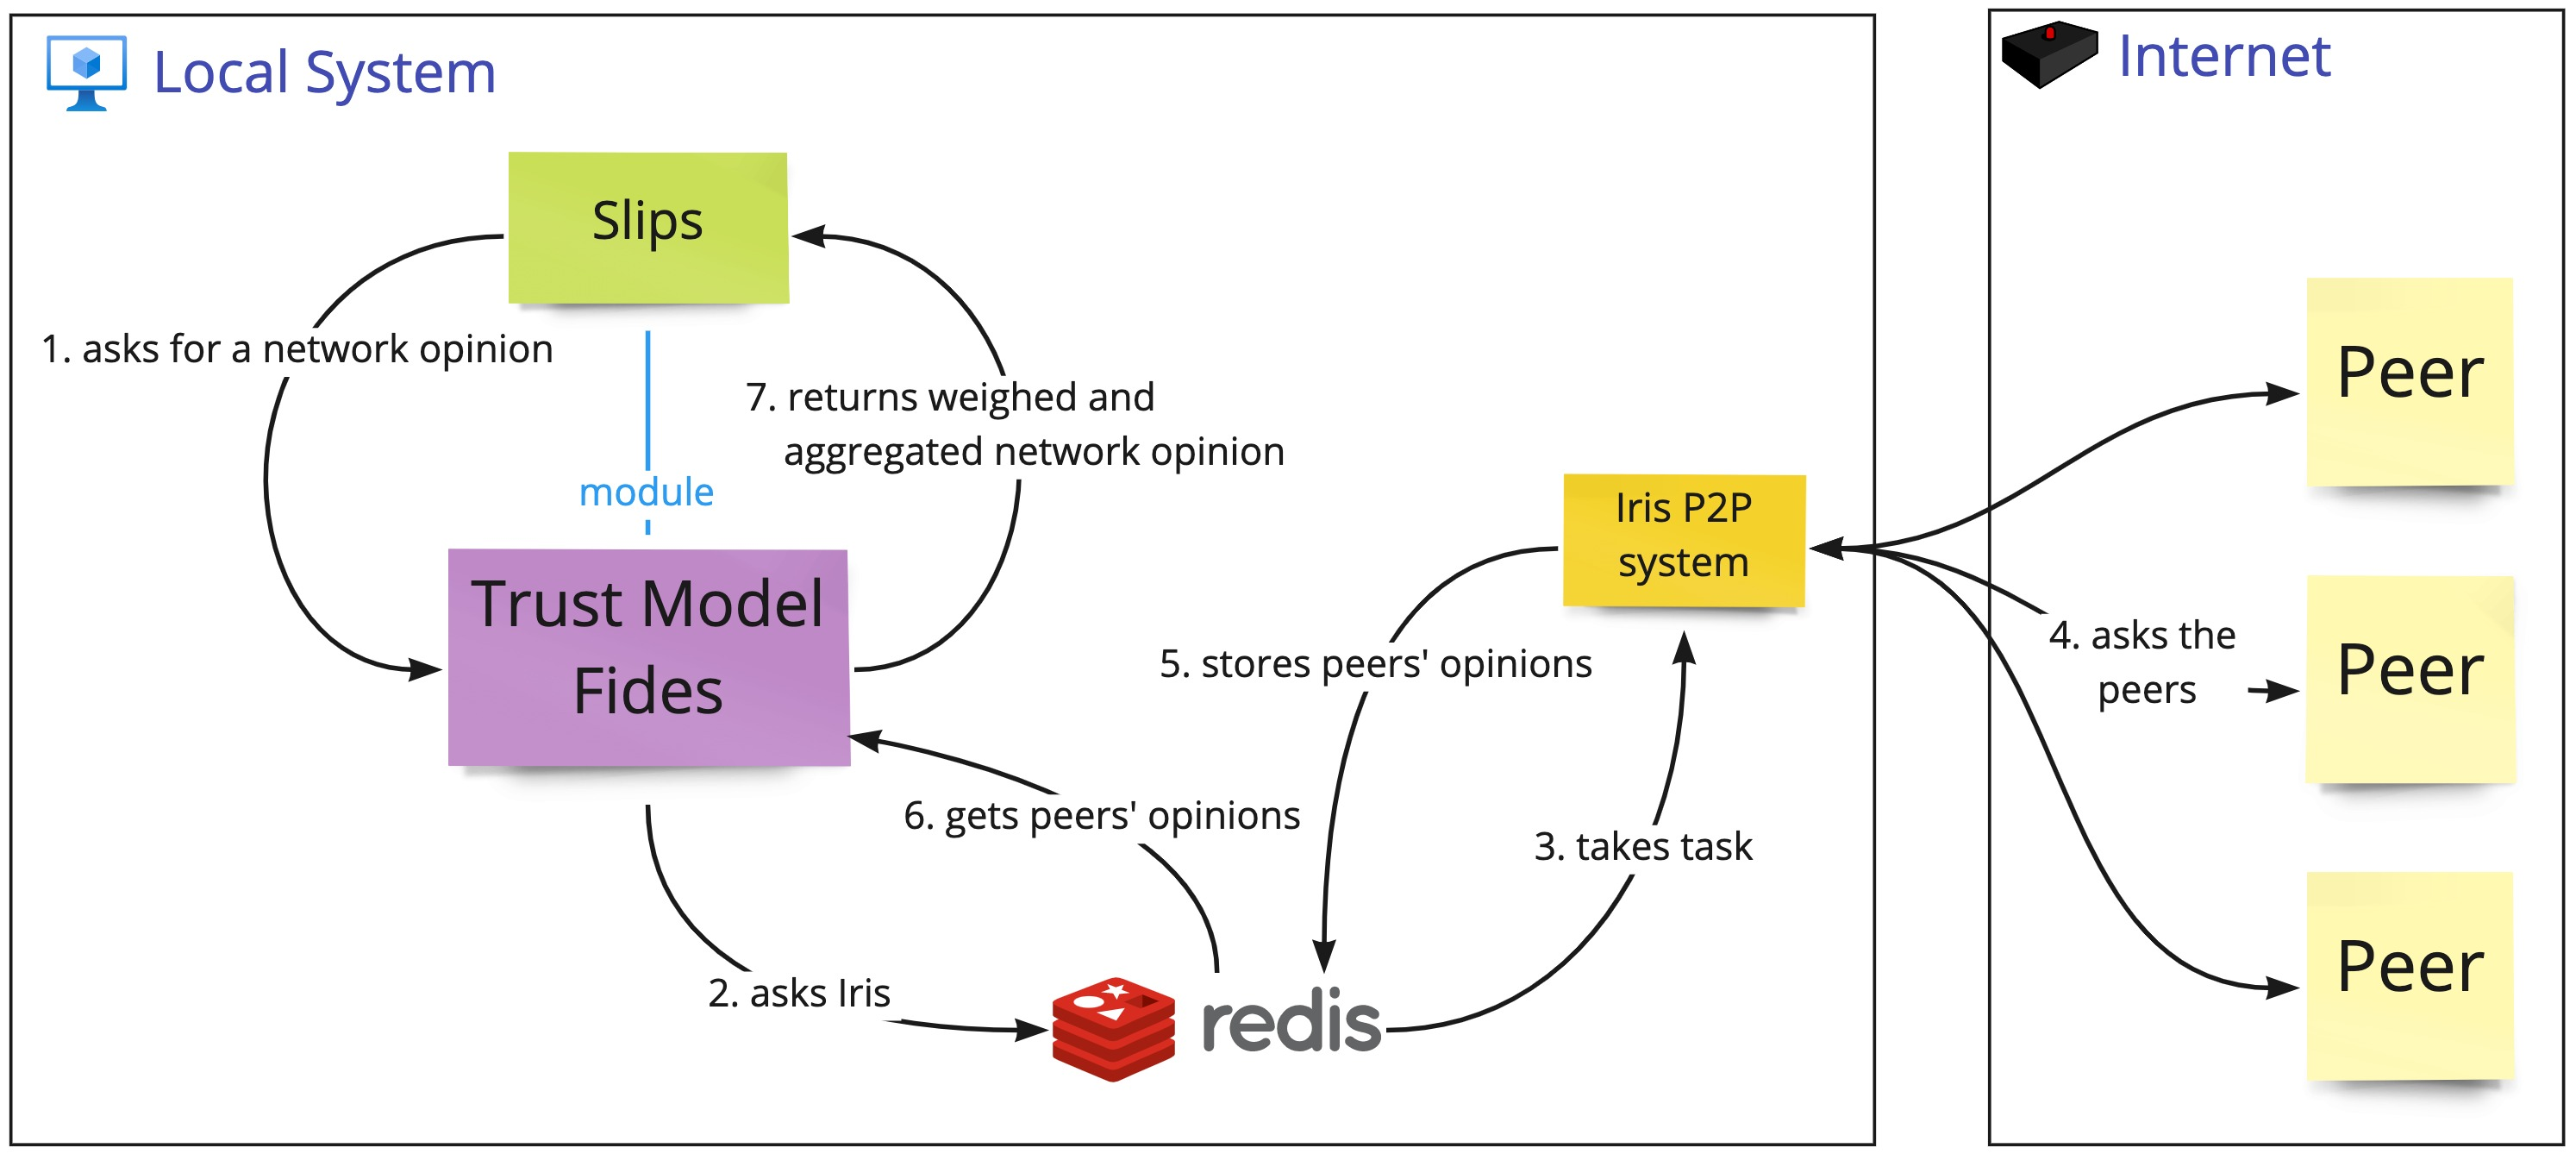
\includegraphics[width=1.0\textwidth]{assets/communication_architecture.jpeg}
    \caption{Communication between Fides, Iris and Slips}
    \label{fig:fides-api-network}
\end{figure}

Fides itself is a trust model, set of equations and a data storage for interaction history. 
It does not interact with the network directly, but rather it exposes an API that can be used either to receive the information from the network or for sending the requests back to the network.
Thanks to this design, where all business logic is separated from the network layer, Fides is highly modular and it does not depend on the network layer implementation.
The network layer Iris then performs all data transfers and facilitates all communications with the remote peers.
It also facilitates finding new peers and ensuring that all requests from Fides are dispatched to the correct recipients.
In the eyes of Fides, the network layer is a \textit{black box} and it does not need to know, how is the network layer implemented.
See the figure~\ref{fig:fides-api-network} for a high-level overview of the communication.

The network layer, \textbf{Iris}, was developed by Bc. Martin Řepa in~\cite{nl} where Řepa describes how Iris works in detail and what protocols are used to safely deliver necessary information and messages between the instances of Fides.

\section{Implementation}
\label{sec:implementation}
Because Fides was designed to integrate with Slips, we were constrained by Slips implementation and thus Fides is implemented in Python 3.8.

The code is versioned by git and published on GitHub in repository \href{https://github.com/LukasForst/fides}{github.com/LukasForst/fides}~(\cite{fidesGithub}).
We choose to use Conda \cite{conda} for managing dependencies and Python versions.

\subsection{Configuration}
\label{subsec:configuration}
Our trust model contains many different configuration options either related to the computational model itself or to the data persistence or identity of the local peer.

Computational model settings are for example threat intelligence aggregation methods described in the section \ref{sec:network-intelligence-aggregation} or interaction evaluation strategy from the section \ref{sec:interaction-evaluation-strategies}.
As the trust model needs only a single method, the administrator needs to define which one of these functions should be used.

The configuration itself is in a single YAML \cite{yaml} format in \href{https://github.com/LukasForst/fides/blob/master/fides.conf.yml}{\textit{fides.conf.yml}}~(\cite{fidesGithub}) file.
This file is loaded and validated during the trust model startup and is used to provide all possible configuration options for the trust model.

\subsection{Persistence}
\label{subsec:persistence}
Fides stores trust-related data such as past interactions, cached network opinions, service trust, recommendations, etc. inside the database.
The database layer was implemented as an abstract part and can be easily replaced in the future.
As of now, we have two different implementations - an in-memory database and a database that stores data in Redis, if the persistence is needed.
However, thanks to its modularity, any other persistence solution can be implemented in the future.

\subsection{Data Filtering}
\label{subsec:data-filtering}
Part of the configuration is the section about data confidentiality and sharing of the threat intelligence with other peers.
Fides allows operators to choose what threat intelligence will be shared when and to who.

For example, if the threat intelligence received from the local Slips instance contains a  \textit{confidentiality level}, the operator can enforce that only peers with \textit{high} service trust will receive this threat intelligence when they ask for it.

Confidentiality level, $0 \leq cl \leq 1$, defines how sensitive or confidential the threat intelligence is where $cl = 0$ means public information that can be shared with anybody and $cl = 1$ secret information that should not be shared at all.

Fides administrator can then in configuration ~(\ref{subsec:configuration}) specify what service trust $st$ is required for what confidentiality level $cl$.
If this configuration is in place, whenever remote peer ($j$) asks for the threat intelligence and local ($i$) Slips has requested threat intelligence, Fides verifies that $st_{i, j} \geq cl$ before providing the intelligence to the remote peer.

This mechanism ensures that Slips does not leak information that is private or somehow more sensitive than the others.